\chapter{Taxonomy of Charmed Mesons}

\epigraph{\textitalian{All'inizio, l'arte del puzzle sembra un'arte breve, di poco spessore, tutta contenuta in uno scarno insegnamento della \emph{Gestalttheorie}: l'oggetto preso di mira---sia esso un atto percettivo, un apprendimento, un sistema fisiologico o, nel nostro caso, un puzzle di legno---non è una somma di elementi che bisognerebbe dapprima isolare e analizzare, ma un insieme, una forma cioè, una struttura: l'elemento non preesiste all'insieme, non è più immediato ne più antico, non sono gli elementi a determinare l'insieme, ma l'insieme a determinare gli elementi: la conoscenza del tutto e delle sue leggi, dell'insieme e della sua struttura, non è deducibile dalla conoscenza delle singole parti che lo compongono: la qual cosa significa che si può guardare il pezzo di un puzzle per tre giorni di seguito credendo di sapere tutto della sua configurazione e del suo colore, senza aver fatto il minimo passo avanti: conta solo la possibilità di collegare quel pezzo ad altri pezzi e in questo senso l'arte del puzzle e l'arte del go hanno qualcosa in comune; solo i pezzi ricomposti assumeranno un carattere leggibile, acquisteranno un senso: isolato, il pezzo di un puzzle non significa niente; è semplicemente una domanda impossibile, sfida opaca; ma se appena riesci, dopo molti minuti di errori e tentativi, o in un mezzo secondo prodigiosamente ispirato, a connetterlo con uno dei pezzi vicini, ecco che quello sparisce, cessa di esistere in quanto pezzo: l'intensa difficoltà che ha preceduto l'accostamento e che la parola \emph{puzzle}---enigma---traduce così bene in inglese, non solo non ha più motivo di esistere, ma sembra non averne avuto mai, tanto si è fatta evidenza: i due pezzi miracolosamente riuniti sono diventati ormai uno, a sua volta fonte di errori, esitazioni, smarrimenti e attesa.}}{(George Perec, \emph{La Vie mode d'emploi})}

In the first chapter it was seen that different open-charm meson states and some open-beauty ones have been observed and, thanks to LHCb and BelleII, one expects that as time goes by these spectra will become more and more populated. In the second chapter it was introduced a theoretical framework inspired by QCD which on one hand allows to classify the heavy-light mesons and on the other to describe their low-energy strong interactions with light pseudoscalar mesons in terms of a small number of unknown constants (which in principle should be obtained in some other way, e.g. experimentally). In this chapter, such theory is used for the classification of established and recently observed open-charm mesons according to its scheme \cite{Colangelo:2012xi}. Moreover, the decay widths of these states (with respect to selected decay modes) will be calculated within this theory and it will be shown how the result can be used to make model-independent predictions of their quantum numbers.

\section{Strong Two-body decays to the Fundamental Doublet}

%\begin{table}
%  \centering
%  \begin{tabular}{c c c c c c c c}
%    \toprule
%    & & \multicolumn{2}{c}{$c \adj{q}$} & \multicolumn{2}{c}{$c \adj{s}$} & $b \adj{q}$ & $b \adj{s}$  \\
%    Doublet & $J^P$ & $n_r = 1$ & $n_r = 2$ & $n_r = 1$ & $n_r = 2$ & $n_r = 1$ & $n_r = 1$ \\
%    \midrule
%    $H$ & $0^-$ & $D(1869)$ & $\left. D(2550) \right.^\star$ & $D_s(1968)$ & & $ B(5279)$ & $ B_s(5366)$ \\ 
%    $H$ & $1^-$ & $D^*(2010)$ & $\left. D^* (2600) \right.^\star$ & $D_s^*(2112)$ & $D_{s1}^*(2700)$ & $ B^*(5325)$ & $ B_s^*(5415)$ \\
%    \addlinespace
%    $S$ & $0^+$ & $D^*_0(2400)$ & & $D_{s0}^*(2317)$ & & & \\
%    $S$ & $1^+$ & $D'_1(2430)$ & & $D'_{s1}(2460)$ & $\left. D_{sJ}(3040) \right.^\star$ & & \\
%    \addlinespace
%    $T$ & $1^+$ & $D_1(2420)$ & & $D_{s1}(2536)$ & $\left. D_{sJ}(3040) \right.^\star$ & $ B_1(5721)$ & $B_{s1}(5830)$ \\
%    $T$ & $2^+$ & $D^*_2(2460)$ & $\left. D^*_2(3000) \right.^\star$ & $D_{s2}^*(2573)$ & & $ B_2^*(5747)$ & $ B_{s2}^*(5840)$ \\
%    \addlinespace
%    $X$ & $1^-$ & & & $D^*_{s 1}(2860)$ & & & \\
%    $X$ & $2^-$ & & & & & & \\
%    \addlinespace
%    $X'$ & $2^-$ & $\left. D(2750) \right.^\star$ & & & & & \\
%    $X'$ & $3^-$ & $D^*_3(2760)$ & & $D^*_{s 3}(2860)$ & & & \\
%    \addlinespace
%    $F$ & $2^+$ & $\left. D^*_2(3000) \right.^\star$ & & & & & \\
%    \bottomrule
%  \end{tabular}
%  \caption{Observed open-charm and open-beauty mesons, classified in HQ doublets. States with uncertain assignment are indicated with $\star$.}
%  \label{tab:charm}
%\end{table}

I will recall some basic facts. The classification of heavy mesons is based on the quantum numbers of the light degrees of freedom (light quark plus gluons) and of the heavy quark, which decouples from the former due to its large mass. Therefore a state is characterized by the orbital angular momentum of the light degrees of freedom $L$, by their total angular momentum $S_\ell$ and by the meson spin $J$. Their parity will be $P = (-1)^{L + 1}$ and for each value of $S_\ell$ there will be two possible doublets of states with opposite parity, vice versa given $S_\ell^P$ there is only one possible value of $L$. The two states of each doublet are degenerate in the exact HQ limit, they correspond to the two possible orientations of the heavy meson spin and have different $J$. More than one state with any given combination of these quantum numbers can exist and accounts for radial excitations identified by increasing radial quantum number $n$.

In the first place, the classification of states is done according to their quantum number and mass, i.e. a resonance with given $J^P$ is a candidate for the lowest vacant states with that quantum numbers (which could have $n > 1$). However, apart for the $J = 0$ state, for each value of $J^P$ there exist two series of doublets, with respectively $S_l = \left( J - 1/2 \right)^P \text{ and } \left( J + 1/2 \right)^P$, that contain a state with the given $J^P$. To distinguish between these two series it is necessary to use an additional piece of information, which is carried by the width of the state.

As reviewed in section \ref{sec:heavy_ChPT}, in heavy ChPT it is possible to write effective Lagrangian terms that describe the strong decays of a heavy meson in a given doublet to another heavy meson in a second doublet with the emission of a light pseudoscalar meson. Eqs \ref{eqs:HChPT_interaction_Lagrangians} refer to the case in which the meson in the final state belongs to the fundamental doublet $H$. Each Lagrangian is weighted by a strong coupling constant that cannot be fixed within the same approach, so that it is in principle unknown. However, it should be stressed that a single parameter (i.e. the strong coupling constant) can describe (if allowed) four possible decays, corresponding to the two possible decaying mesons in the initial state doublet and two possible final state mesons in the other doublet. Therefore, such a parameter cancels in  the ratio of two strong decay rates computed from the same effective Lagrangian term. As a consequence, such ratios represent model independent predictions of the method.

Exploiting this approach, in the following I focus on the decays of a meson in a generic doublet $M$ to another one in the fundamental doublet $H$ with emission of a light pseudoscalar meson generically denoted as $\pi$. The reason of this lies in the large phase space available for these models and in the relative simplicity of their reconstruction in experimental analysis. The kinematics of the decays $M \to H \pi$ is that of a standard two body decay and its width can be written as
\begin{equation}
  \D \! \Gamma= \frac{1}{32 \pi^2} \left\vert \left\langle H \left( v \right), \pi \left( q \right) \right\vert T \left\vert M \left( v \right) \right\rangle \right\vert^2 \frac{\left\Vert \symbf{q} \right\Vert}{m_M} \D \! \Omega \ .
  \label{eq:diff_decay_width}
\end{equation}
%where $\symbf{p}'$ and $\epsilon$ are the momentum and polarization tensor of the daughter heavy meson, $\D \! \Omega$ is infinitesimal solid angle of around $\symbf{p}'$, $q$ is the four-momentum of the light pseudoscalar one and $v$, $\eta$ and $m_M$ are respectively the velocity, polarization and mass of the decaying heavy meson. At tree level holds
%\begin{equation}
%  \left\langle H \left( v , \epsilon \right), \pi \left( q \right) \right\vert S \left\vert M \left( v, \eta \right) \right\rangle = \left\langle H \left( v, \epsilon \right), \pi \left( q \right) \right\vert \symcal{L}_{M \text{, Int}} \left\vert M \left( v, \eta \right) \right\rangle \ ,
%\end{equation}
%where, with the normalization convention used, the $M(x)$ field is such that
%\begin{equation}
%  \left\langle 0 \right\vert M^{\mu_1 \cdots \mu_k}(x) \left\vert M(v , \epsilon) \right\rangle = \sqrt{m_M} \ \epsilon^{\mu_1 \cdots \mu_k} \ e^{- i v_\nu x^\nu} \ .
%\end{equation}
%
%Because one is interested in the unpolarized decay width, it is necessary to sum over the final polarization states and average over the initial ones. After these sums, using the relations \eqref{eq:polarization_sums}, the only four vector on which the RHS of the equation \eqref{eq:diff_decay_width} can depend are $v$ and $q$. Therefore, in the frame of reference in which the decaying heavy meson is at rest there is no preferred direction and the differential decay width of equation \eqref{eq:diff_decay_width} has no dependence on $\Omega$. Putting all together, it must be
%\begin{equation}
%  \Gamma= \frac{1}{16 \pi} \ \frac{1}{2 J + 1} \sum_\epsilon \sum_\eta \left\vert \left\langle H \left( v, \epsilon \right), \pi \left( q \right) \right\vert S \left\vert M \left( v , \eta \right) \right\rangle \right\vert^2 \frac{\left\Vert \symbf{p}' \right\Vert}{m_M} \ ,
%\end{equation}
%where $J$ is the spin of the decaying particle.

If the decaying meson has spin $J$ the factor $1/(2 J + 1)$ should be included in the equation \eqref{eq:diff_decay_width} to average over the spin.

$\left\langle H \left( v \right), \pi \left( q \right) \right\vert T \left\vert M \left( v \right) \right\rangle$ is the transition aplitude that can be directly computed from the effective Lagrangian terms. According to the velocity superselection rule, the two heavy mesons in the initial and final state have the same velocity. It is important to notice that this velocity superselection rule is valid only in the calculation of the matrix element and not in the calculation of the phase space that is fixed only by the kinematics.

In the frame of reference in which $M$ is at rest (i.e. $v = (1, \symbf{0})$) one has
\begin{equation}
  \left\Vert \symbf{q} \right\Vert = \frac{\sqrt{\left(m_M^2 - (m_H + m_\pi)^2\right) \left(m_M^2 - (m_H - m_\pi)^2\right)}}{2 m_M} .
\end{equation}

In the following I will list the allowed decays of heavy mesons belonging to one of the doublets introduced in equations \eqref{eq:H_doublet}, \eqref{eq:S_doublet}, \eqref{eq:other_doublets} and write down all the corresponding Lagrangian terms. Moreover, the covariant representation and structure of the interaction Lagrangian of states with $n > 1$ are the same as the corresponding one of the state with $n = 1$ and same $S_\ell^P$. However, the interaction Lagrangian terms for radial excited states have different coupling constants and, in the following, the coupling constant for the first radial excitation is denoted with the same symbol of the corresponding $n = 1$ state and marked by a tilde.

Some of the decay modes for $n = 2$ states of these mesons are explicitly listed in the following, because such decay modes towards doublets with higher $L$ are kinematically prohibited for $n = 1$ states but may be possible for ones with $n > 1$. Finally the Clebsh-Gordan coefficients associated with the light pseudoscalar meson in the final state (and built into the definition of $\symcal{M}$) are explicitly indicated with $C_\pi$.

It should be noticed that, the small $\Vert q \Vert$ behaviour of the decay widths reveal the dominant partial wave contribution to the decay and vice versa if the decay is known to occur in $l$-wave, at small $\Vert q \Vert$ will hold $\Gamma \propto \Vert q \Vert^{2 l+1}$.

\paragraph{Decaying meson $H = \left( P, P^* \right)$ or $\tilde{H} = \left( \tilde{P}, \tilde{P}^* \right)$}
\begin{equation}
  \symcal{L}_{H \text{, Int}} = g \tr{\left(\adj{H}_a H_b \gamma_\mu \gamma^5 A_{ba}^\mu \right)} \ .
\end{equation}
Allowed decays 
\begin{subequations}
  \begin{align}
    \Gamma \left( P^* \to P \pi \right) &= C_\pi \frac{g^2}{6 \pi f_\pi^2} \frac{m_P}{m_{P^*}} \left\Vert \symbf{q} \right\Vert^3 \ , \\
    \Gamma \left( \tilde{P}^* \to P \pi \right) &= C_\pi \frac{\tilde{g}^2}{6 \pi f_\pi^2} \frac{m_P}{m_{\tilde{P}^*}} \left\Vert \symbf{q} \right\Vert^3 \ , \\
    \Gamma \left( \tilde{P}^* \to P^* \pi \right) &= C_\pi \frac{\tilde{g}^2}{3 \pi f_\pi^2}\frac{m_{P^*}}{m_{\tilde{P}^*}} \left\Vert \symbf{q} \right\Vert^3 \ , \\
    \Gamma \left(\tilde{P} \to P^* \pi \right) &= C_\pi \frac{\tilde{g}^2}{2 \pi f_\pi^2} \frac{m_{P^*}}{m_{\tilde{P}}} \left\Vert \symbf{q} \right\Vert^3 \ .
  \end{align}
\end{subequations}

\paragraph{Decaying $S = \left( P^*_0, P'_1 \right)$}
\begin{equation}
  \symcal{L}_{S \text{, Int}} = h \tr{\left(\adj{H}_a S_b \gamma_\mu \gamma^5 A_{ba}^\mu \right)} + \text{h.c.} \ .
\end{equation}
Allowed decays
\begin{subequations}
  \begin{align}
    \Gamma \left( P^*_0 \to P \pi \right) &= C_\pi \frac{h^2}{2 \pi f_\pi^2} \frac{m_P}{m_{P^*_0}} \left\Vert \symbf{q} \right\Vert \left( m_\pi^2 + \left\Vert \symbf{q} \right\Vert^2 \right) \ , \\
    \Gamma \left( P'_1 \to P^* \pi \right) &= C_\pi \frac{h^2}{2 \pi f_\pi^2} \frac{m_{P^*}}{m_{P'_1}} \left\Vert \symbf{q} \right\Vert \left( m_\pi^2 + \left\Vert \symbf{q} \right\Vert^2 \right) \ .
  \end{align}
\end{subequations}

\paragraph{Decaying $T = \left( P_1, P^*_2 \right)$ or $\tilde{T} = \left(\tilde{P}_1, \tilde{P}^*_2 \right)$}
\begin{equation}
  \symcal{L}_{T \text{, Int}} =  \frac{h'}{\Lambda_\chi} \tr{\left(\adj{H}_a T^\mu_b \left( i D_\mu \slashed{A} + i \slashed{D} A_\mu \right)_{ba} \gamma^5 \right)} + \text{h.c.} \ .
\end{equation}
Allowed decays
\begin{subequations}
  \begin{align}
    \Gamma \left( P_1 \to P^* \pi \right) &= C_\pi \frac{2 h^{\prime 2}}{3 \pi f_\pi^2} \frac{m_{P^*}}{ m_{P_1}} \left\Vert \symbf{q} \right\Vert^5 \ , 
    \label{eq:P1toP*pi} \\
    \Gamma \left( P_2^* \to P \pi \right) &= C_\pi \frac{4 h^{\prime 2}}{15 \pi f_\pi^2} \frac{m_P}{m_{P_2^*}} \left\Vert \symbf{q} \right\Vert^5 \ , 
    \label{eq:P2*toPpi} \\
    \Gamma \left( P_2^* \to P^* \pi \right) &= C_\pi \frac{2 h^{\prime 2}}{5 \pi f_\pi^2} \frac{m_{P^*}}{m_{P_2^*}} \left\Vert \symbf{q} \right\Vert^5 \ .
    \label{eq:P2*toP*pi}
  \end{align}
\end{subequations}

\paragraph{Decaying $X = \left( P_1^* , P_2 \right)$}
\begin{equation}
  \symcal{L}_{X \text{, Int}} = \frac{k'}{\Lambda_\chi} \tr{\left( \adj{H}_a X^\mu_b \left( i D_\mu \slashed{A} + i \slashed{D} A_\mu \right)_{ba} \gamma^5 \right)} + \text{h.c.} \ .
\end{equation}
Allowed decays
\begin{subequations}
  \begin{align}
    \Gamma \left( P^*_1 \to P \pi \right) &= C_\pi \frac{4 k^{\prime 2}}{9 \pi f_\pi^2} \frac{m_P}{m_{P^*_1}} \left\Vert \symbf{q} \right\Vert^3 \left( m_\pi^2 + \left\Vert \symbf{q} \right\Vert^2 \right) \ , \\
    \Gamma \left( P^*_1 \to P^* \pi \right) &= C_\pi \frac{2 k^{\prime 2 }}{9 \pi f_\pi^2} \frac{m_{P^*}}{m_{P^*_1}} \left\Vert \symbf{q} \right\Vert^3 \left( m_\pi^2 + \left\Vert \symbf{q} \right\Vert^2 \right) \ , \\
    \Gamma \left( P_2 \to P^* \pi \right) &= C_\pi \frac{2 k^{\prime 2}}{3 \pi f_\pi^2} \frac{m_{P^*}}{m_{P_2}} \left\Vert \symbf{q} \right\Vert^3 \left( m_\pi^2 + \left\Vert \symbf{q} \right\Vert^2 \right) \ . \\
  \end{align}
\end{subequations}

\paragraph{Decaying $X' = \left( P_2, P^*_3 \right)$}
\begin{multline}
  \symcal{L}_{X' \text{, Int}} =  \frac{1}{\Lambda_\chi^2} \tr \left( \adj{H}_a X^{\prime \mu \nu}_b \left( k_1 \left( D_\mu D_\nu A_\lambda + D_\nu D_\mu A_\lambda \right) \right. \right. \\ +  \left. \left. k_2 \left( D_\mu D_\lambda A_\nu + D_\nu D_\lambda A_\mu \right) \right)_{ba}  \gamma^\lambda \gamma^5 \right) + \text{h.c.} \ .
\end{multline}
Allowed decays
\begin{subequations}
  \begin{align}
    \Gamma \left( P_2 \to P^* \pi \right) &= C_\pi \frac{4 k^2}{15 \pi f_\pi^2} \frac{m_{P^*}}{m_{P_2^{\prime *}}} \left\Vert \symbf{q} \right\Vert^7 \ , \\
    \Gamma \left( P^*_3 \to P \pi \right) &= C_\pi \frac{4 k^2}{35}{f_\pi^2} \frac{m_{P}}{m_{P^*_3}} \left\Vert \symbf{q} \right\Vert^7 \ , \\
    \Gamma \left( P^*_3 \to P^* \pi \right) &= C_\pi \frac{16 k^2}{105 \pi f_\pi^2} \frac{m_{P^*}}{m_{P^*_3}} \left\Vert \symbf{q} \right\Vert^7 \ ,
  \end{align}
\end{subequations}
with $k = k_1 + k_2$.

\paragraph{Decaying $F = \left( P^{* \prime}_2, P_3 \right)$}
\begin{multline}
  \symcal{L}_{F \text{, Int}} =  \frac{1}{\Lambda_\chi^2} \tr \left( \adj{H}_a F^{\mu \nu}_b \left( l_1 \left( D_\mu D_\nu A_\lambda + D_\nu D_\mu A_\lambda \right) \right. \right. \\ +  \left. \left. l_2 \left( D_\mu D_\lambda A_\nu + D_\nu D_\lambda A_\mu \right) \right)_{ba}  \gamma^\lambda \gamma^5 \right) + \text{h.c.} \ .
  \label{eq:F_Lagrangian}
\end{multline}
Allowed decays
\begin{subequations}
  \begin{align}
    \Gamma\left( P_2^{* \prime} \to P \pi \right) &= C_\pi \frac{4 l^2}{25 \pi f_\pi^2 \Lambda_\chi^4} \frac{m_P}{m_{P_2^{* \prime}}} \Vert \symbf{q} \Vert^5 \left( m^2_\pi + \Vert \symbf{q} \Vert^2 \right) \ , 
    \label{eq:P2*'toPpi} \\
    \Gamma\left( P_2^{* \prime} \to P^* \pi \right) &= C_\pi \frac{8 l^2}{75 \pi f_\pi^2 \Lambda_\chi^4} \frac{m_P^*}{m_{P_2^{* \prime}}} \Vert \symbf{q} \Vert^5 \left( m^2_\pi + \Vert \symbf{q} \Vert^2 \right) \ , 
    \label{eq:P2*'toP*pi} \\
    \Gamma\left( P_3 \to P^* \pi \right) &= C_\pi \frac{4 l^2}{105 \pi  f_\pi^2 \Lambda_\chi^4} \frac{m_{P^*}}{m_{P_3}} \left\Vert \symbf{q} \right\Vert^5 \left( 7 m_\pi^2 + 4 \left\Vert \symbf{q} \right\Vert^2 \right) \ ,
    \label{eq:P3toP*pi}
  \end{align}
\end{subequations}
with $l = l_1 + l_2$.

\section{Classification of Established States}

The established states of the open-charm meson spectrum are listed in table \ref{tab:charm_taxonomy} (together with the recently observed ones according to the classification proposed in this thesis) and, to give a bird's eye view, one could say that these states fill the $H$, $S$ and $T$ doublets. In the following I give an overview of their classification in some detail.

%The two states belonging to the fundamental doublet, with $S_\ell^P = 1/2^-$ and $n = 1$, are well known, both in the strange and non-strange sector (actually, the same is true for the open-beauty spectrum): the fundamental state is by definition the lightest $D_{(s)}$ meson and have $J^P = 0^-$ , the $D^*_{(s)}$ is the lightest $J^P = 1^-$ meson and decay through $p$-wave to $D_{(s)}$, all of their properties are in accord with the quark model for both neutral (without strangeness) and charged (with and without strangeness) versions. Therefore, this discussion will mainly concern the excited doublets with $S_\ell^P = \left. 1/2 \right.^+ , \left. 3/2 \right.^-, \cdots$ and/or $n > 1$. 

The fundamental doublet with $S_\ell^P = 1/2^-$ and $n = 1$ is filled by the well known states both in the strange and non-strange sector: the lightest $D_{(s)}$ meson with $J^P = 0^-$ and the $D^*_{(s)}$ meson with $J^P = 1^-$ meson; their properties are in agreement with quark model for both neutral and charges states.

If one looks at the observations of the open-charm and open-beauty states from a historical perspective, it is easy to spot a pattern in which states of the $T$ doublet are the first to be observed after the fundamental ones. This should cause no surprise: although the states of the $S$ doublet are lighter than those of the $T$ doublet (as expected by the quark model), the former have broad widths since they decay through $s$-wave and therefore they are more difficult to observe than the latter, which decay through $d$-wave and thus are rather narrow. Indeed, the $S_\ell^P = \left. 3/2 \right.^+$ states with $J^P = 1^+ \text{ and } 2^+$ are filled respectively by the $D_1(2420)$ and the $D^*_2(2460)$ in the non-strange sector and by the $D_{s1}(2536)$ and by the $D^*_{s 2}(2573)$ in the strange one.

The non-strange states with $S_\ell^P = \left. 1/2 \right.^+$ and $n = 1$ and are filled by the $D^*_0(2400)$ and by the $D'_1(2430)$, which have large widths and are the lightest known states with respectively $J^P = 0^+ \text{ and } 1^+$. Notice that the masses of the four states of both the $S$ and $T$ doublets lie in a range of about $100 \ \text{MeV}$, which is small compared to the splitting with respect to the $H$ doublet ($\approx 350 \ \text{MeV}$): this can be justified in light of the quark model because the $S$ and $T$ doublets have both $L = 1$ while $H$ has $L = 0$.

The case of charmed mesons with strangeness is more convoluted. As noticed in the first chapter, the mass of the $D^*_0(2317)$ and of the $D'_1(2460)$ are much smaller than suggested by the quark model for this doublet. This led to the speculation that these states may contain four quarks, either as tetraquark or as molecule formed by $D$ and $K$ mesons. The tetraquark picture predicts a large number of states, which were not observed by further search of the \textsc{BaBar} and Belle collaborations in the mass region of the $D^*_{s 0}$, hence making this picture disfavoured. Moreover, the masses of the $D^*_{s 0}$ and the $D_{s 1}$ are just below the threshold of $D K$ and $D^* K$ respectively, which accounts for the small widths of these states (unexpected for $S$ doublet states) since they are forced to decay violating isospin. This has suggested that these two states could be hadronic molecules or mixtures of hadronic molecules and ordinary $c \adj{s}$ mesons. However, theoretical predictions for their (isospin violating) hadronic and radiative decays \cite{Colangelo:2003vg,Colangelo:2005hv} strongly support their identification with the ordinary $c \adj{s}$ mesons belonging to the $S$ doublet.

The only remaining established state without strangeness is the $D^*_3(2760)$, also known as $D^*(2760)$ or $D(2750)$ in the PDG nomenclature. This state was known to have natural parity since its observation by \textsc{BaBar} (it decays to $D \pi$) and its spin-parity was later fixed by LHCb. Possible states with $J^P = 3^-$ and $n = 1$ are those belonging to $X'$ doublet, which has $L = 2$, and to a higher doublet with $L = 4$ (not considered in this thesis); however,the latter is expected to have much larger mass and so the $D^*_3(2760)$ is reasonably identified with the former.

The $D_{s J}(2860)$ and $D^*_{s 1}(2700)$ were observed both in the $D K$ and $D^* K$ channels by Belle and \textsc{BaBar} and later confirmed by LHCb. The spin-parity of $D^*_{s 1}(2700)$ was established by production studies, finding $J^P = 1^-$. Measurements of branching ratios and criteria based on heavy ChPT (analogous to those object of this thesis) suggested the identification with the $\tilde{D}^*_{s 1}$ \cite{Colangelo:2007ds}, the first radial excitation of the $D^*_s(2112)$. 

The common history of the $D^*_{s 1}(2860)$ and the $D^*_{s 3}(2860)$ dates back to an observation by the \textsc{BaBar} collaboration, indicated as the $D_{s J}(2860)$, the identification of which constituted a puzzle \cite{Colangelo:2012xi}. In \cite{Colangelo:2006rq} the identification of the $D^*_{s 3}(2860)$ with the state having $J^P = 3^-$ belonging to the $X'$ was proposed and later confirmed by LHCb \cite{Aaij:2014xza}. After that, $D^*_3(2760)$ was recognized as the non-strange partner of the $D^*_{s 3}(2860)$. The case of the $D^*_{s 1}(2860)$ is more uncertain and therefore is postponed in the following paragraph.

%\begin{table}
%  \centering
%  \small
%  \begin{tabular}{c c c c c c}
%    \toprule
%     & & & & \multicolumn{2}{c}{World averages} \\ 
%    \textsc{BaBar} (2010) & LHCb (2013) & LHCb (2016) & PDG & mass (MeV) & $\Gamma$ (MeV) \\ 
%    \midrule
%    $D(2550)$ & $D_J(2580)$ & & $D(2550)$ & $2564 \pm 20$  & $135 \pm 17$ \\
%    $D^*(2600)$ & $D^*_J(2650)$ & & $D^*_J(2600)$ & $2623 \pm 12$ & $139 \pm 31$ \\
%    $D^*(2760)$ & $D^*_J(2760)$ & & $D(2750)$ & $2763.5 \pm 3.4$ & $66 \pm 5$ \\
%    \bottomrule
%  \end{tabular}
%  \caption{Matching of nonestablished open-charm mesons by PDG.}
%  \label{tab:LHCb2013}
%\end{table}

\begin{table}
  \centering
  \footnotesize
  \begin{tabular}{c c c c c c c c}
    \toprule
    & & \multicolumn{3}{c}{$c \adj{q}$} & \multicolumn{3}{c}{$c \adj{s}$} \\
    Doublet & $J^P$ & $n = 1$ & $n = 2$ & $n = 3$ & $n = 1$ & $n = 2$ & $n = 3$ \\
    \midrule
    $H$ & $0^-$ & $D(1869)$ & $\left. D(2550) \right.^\star$ & & $D_s(1968)$ & & \\ 
    $H$ & $1^-$ & $D^*(2010)$ & $\left. D^* (2600) \right.^\star$ & $\left. D^*_1(2680) \right.^\star$ & $D_s^*(2112)$ & $D_{s1}^*(2700)$ & $\left. D^*_{s 1}(2860) \right.^\star$ \\
    \addlinespace
    $S$ & $0^+$ & $D^*_0(2400)$ & & & $D_{s0}^*(2317)$ & & \\
    $S$ & $1^+$ & $D'_1(2430)$ & $\left. D(3000) \right.^\star$ & & $D'_{s1}(2460)$ & $\left. D_{sJ}(3040) \right.^\star$ & \\
    \addlinespace
    $T$ & $1^+$ & $D_1(2420)$ & $\left. D(3000) \right.^\star$ & & $D_{s1}(2536)$ & $\left. D_{sJ}(3040) \right.^\star$ & \\
    $T$ & $2^+$ & $D^*_2(2460)$ & & & $D_{s2}^*(2573)$ & & \\
    \addlinespace
    $X$ & $1^-$ & $\left. D^*_1(2680) \right.^\star$ & & & $\left. D^*_{s 1}(2860) \right.^\star$ & & \\
    $X$ & $2^-$ & & & & & & \\
    \addlinespace
    $X'$ & $2^-$ & $\left. D(2750) \right.^\star$ & & & & & \\
    $X'$ & $3^-$ & $D^*_3(2760)$ & & & $D^*_{s 3}(2860)$ & & \\
    \addlinespace
    $F$ & $2^+$ & $\left. D^*_2(3000) \right.^\star$ & & & & & \\
    $F$ & $3^+$ & & & & & & \\
    \bottomrule
  \end{tabular}
  \caption{Observed open-charm mesons, classified in HQ doublets. States with uncertain identification are indicated with $\star$.}
  \label{tab:charm_taxonomy}
\end{table}

\section{Discussion of States of Uncertain Classification}

At present, the non-strange states with uncertain classification are the $D(2550)$ \cite{delAmoSanchez:2010vq,Aaij:2013sza}, the $D^*(2600)$ \cite{delAmoSanchez:2010vq}, the $D^*_J(2650)$ \cite{Aaij:2013sza,Aaij:2016fma}, the $D(2750)$ \cite{delAmoSanchez:2010vq}, the $D(3000)$ \cite{Aaij:2013sza} and the $D^*_2(3000)$ \cite{Aaij:2013sza,Aaij:2016fma}; while the strange ones are the $D^*_{s 1}(2860)$ \cite{Aaij:2014xza} and $D^*_{s J}(3040)$ \cite{Aubert:2009wg}.

\subsection{State Classification Discussed in the Literature}

As of their first observation, the \textsc{BaBar} collaboration suggested that the $D(2550)$ and the $D^*(2600)$ could belong to the $\tilde{H}$ doublet, i.e. with $S^P_\ell = \left. 1/2 \right.^-$ and $n = 2$, respectively with $J^P = 0^+$ and $1^-$. Hence these states are likely to be identified with the first radial excitations of $(D,\ D^*)$. The $D(2750)$ is regarded as the spin partner of the $D^*(2760)$, thus having $J^P = 2^-$. Comparison with quark model results corroborates these identifications (for a discussion see \cite{Colangelo:2012xi}).

The decay of $D_{sJ}(3040)$ to DK has not been observed, therefore unnatural parity assignment is highly favoured. The lightest not yet observed states of this series are the two $J^P = 2^-$ states with $L = 2$ and $n = 1$, the $3^+$ of the $F$ doublet and the two $J^P = 1^+$ states with $L = 1$ and $n = 2$. The two $2^-$ states are expected to be broader, while the $3^+$ to be heavier. Therefore the $D_{s J}(3040)$ is one of the two axial mesons\footnote{Since this particle has such a large, several decay modes are possible. In particular to decays to $D K^*$ and $D_s \phi$ should allow to discriminate between the $\tilde{D}_{s 1}$ and the $\tilde{D}'_{s 1}$, since the corresponding branching ratios are larger for the latter.} \cite{Colangelo:2010te}.

\subsection{State Classification Proposed in this Thesis}

The remaining states still requiring identification are those observed by LHCb in 2013 \cite{Aaij:2013sza} and 2016 \cite{Aaij:2016fma}. Among the latter, the $D_3^*(2760)$ can be identified with one of the previous observations, indeed it has the same $J^P$ of the $D(2750)$ (using the PDG nomenclature) and compatible mass and width, so it is excluded from further considerations. On the other hand, the identification of the $D(3000)$, $D_1^*(2680)$ and $D_2^*(3000)$ is uncertain. In the remaining of this section I propose a classification of these mesons, which still lacks in the literature.

The $D_1^*(2680)$ could be the $D^*_J(2650)$ seen by the LHCb collaboration in 2013 \cite{Aaij:2013sza}, which has natural parity and similar mass and width. This state could be a higher radial excitation of the fundamental doublet, possibly with $n = 3$, as far as the $D^*(2600)$ is correctly identified with the $n = 2$ one. Another possibility is the identification with the $1^-$ state of the $X$ doublet, both of which states are vacant. 

At first sight, the mass of the $D^*_1(2680)$ does not exclude neither of these identifications. On one hand, if this state belongs to the $X$ doublet, one would expect it to have a mass between the masses of the mesons in the $T$ doublet ($\approx 2450 \ \text{MeV}$) and in the $X'$ ($\approx 2750 \ \text{MeV}$). Therefore $\approx 2.68 \ \text{GeV}$ would be a plausible value. On the other hand, heuristic arguments suggest that the same mass would be compatible with a $n = 3$ state. At the present, no states with $n = 3$ have been identified and hence the mass splitting with respect to the ones with $n = 2$ is not known. However, such mass splitting is expected to be smaller than the one between corresponding pairs of $n = 2$ and $n = 1$ states. Moreover, given the mass difference between the $n = 1$ and $n = 2$ observed states, which is tipically about $500 \ \text{MeV}$, as a crude estimate, a hydrogen-like behaviour with masses proportional to $1/n^2$ would suggest that the separation between states with $n = 2 \text{ and } 3$ would be about $90 \ \text{MeV}$. This estimate is compatible with the observed mass of the $D_1^*(2680)$. Finally, both the $1^-$ states of the $\tilde{H}$ and $X$ doublets are expected to decay in $p$-wave and therefore neither of the alternatives can be ruled out as implausible on the basis of the width of the $D^*_1(2680)$ (which, by the way, is rather broad, about $180 \ \text{MeV}$).

However, further conclusions can be drawn, by taking in consideration the identification of the $D^*_{s 1}(2860)$. The case for this state mirrors the one of the $D^*_1(2680)$: possible identifications are with the vector meson of the $X$ doublet with $n = 1$ and with the one of the $H$ doublet with $n = 3$. Leaving alone the anomalous case of the $D^*_{s 0}(2317)$ and $D'_{s 1}(2460)$, as already noticed, the mass difference between corresponding strange and non-strange states is about $100 \ \text{MeV}$. But the mass difference between the $D_1^*(2680)$ and the $D^*_{s 1}(2860)$ is about $200 \ \text{MeV}$, therefore is likely that the assignment to doublets with the same $S^P_\ell$ are mutually exclusive. The possible scenarios are: $D^*_1(2680)$ belongs to the $X$ doublet with $n = 1$ and $D^*_{s 1}(2860)$ to the $H$ doublet with $n = 3$ or the other way around. It is remarkable that in every case one of the two states has $n = 3$, which if confirmed would be the first of such states.

The identification of the $D(3000)$ is more complicated, being known only that it has unnatural parity. However, due to its large mass, several identifications are unlikely. As will be shown in the following, the $D^*_2(3000)$ is likely to be the $2^+$ state of the $F$ doublet and its mass is larger than the one of the $D(3000)$ by more than $200 \ \text{MeV}$, hence, if the $D(3000)$ is the $3^+$ state of the $F$ doublet there would be a mass inversion and therefore this identification is precluded. Instead, if it is the $2^-$ of the $X$ doublet it would be expected to have mass between the ones of the states of the $T$ and $X'$ doublet, which are sensibly less than $3 \ \text{GeV}$. Therefore also this identification is unlikely. The remaining possibilities are the $n = 3$ and $J^P = 0^-$ state of the $H$ doublet\footnotemark{} and the following three $n = 2$ states: the $2^-$ state of the $X'$ doublet, and the two $1^+$ states. Notice that, in the last scenario, the $D(3000)$ would be the non-strange partner of the $D_{s J}(3040)$ and indeed it has a mass about $100 \ \text{MeV}$ smaller than such state. Moreover, always in this scenario, its mass would be about $500 \ \text{MeV}$ greater than the corresponding $n = 1$ state. Overall, this hypothesis seems to fit nicely with the available data and thus is reported in table \ref{tab:charm_taxonomy}.
\footnotetext{ Notice that, if the $D^*_1(2680)$ is the $n = 3$, $J^P = 1^-$ state, in this scenario there would be a mass inversion within this doublet, therefore this assignment would be ruled out.}

\section{The Classification of the $D^*_2(3000)$}

In this section I present my original contribution aiming at providing all possible ingredients to properly identify the $D^*_2(3000)$, as well as its yet unobserved strange partner.

The $D_2^*(3000)$ could be the $D^*(3000)$ observed by LHCb in 2013 \cite{Aaij:2013sza}, however, as noticed in the 2016 LHCb analysis, the unquoted systematic errors of the 2013 study makes uncertain this identification. Moreover, in the study \cite{Aaij:2013sza} the LHCb collaboration had already put forward the possibility that the observed $D^*(3000)$ could be a superposition of several states in that mass region. Overall, although both states have the same parity and lie in the same mass region (at the edge of the spectrum of observed states), the $D_2^*(3000)$ could be considered a newly observed $D$ meson. 

Having $J^P = 2^+$, the $D^*_2(3000)$ could belong to the $F$ or $\tilde{T}$ doublets, which at the moment are both empty. Moreover, at present, its strange partner is unobserved in both cases. In the following an analysis of the relative branching ratios is proposed to discriminate between the two alternatives, focusing on the neutral state $D^*_2(3000)^0$ which was effectively observed.

%\begin{align}
%  & \tilde{T}^\mu = \frac{1+\slashed{v}}{2} \left\{ \tilde{P}_2^{* \mu \nu} \gamma_\nu - \tilde{P}_{1 \nu} \sqrt{\frac{3}{2}} \gamma_5 \left[ g^{\mu \nu} - \frac{1}{3} \gamma^\nu \left( \gamma^\mu - v^\mu \right) \right] \right\} \\
%  & F^{\mu \nu} = \frac{1 + \slashed{v}}{2} \left\{ P_3^{\mu \nu \rho} \gamma_\rho \gamma_5 - P^{* \prime \alpha \beta}_2 \sqrt{\frac{5}{3}} \left[ \delta^\mu_\alpha \delta^\nu_\beta - \frac{1}{5} \gamma_\alpha \delta^\nu_\beta \left( \gamma^\mu + v^\mu \right) - \frac{1}{5} \gamma_\beta \delta^\mu_\alpha \left( \gamma^\nu + v^\nu \right) \right] \right\}
%\end{align}
%e le lagrangiane di interazione note 
%\begin{align}
%  & \symcal{L}_{\tilde{T}} = \frac{\tilde{h}'}{\Lambda_\chi} \tr{\left[ \adj{H}_a \tilde{T}_b^\mu \left( i D_\mu \slashed{A} + i \slashed{D} A_\mu \right)_{b a} \gamma_5 \right]} + \text{h. c.} \\
%  & \symcal{L}_F = \frac{1}{\Lambda_\chi^2} \tr{\left[ \adj{H}_a F^{\mu \nu}_b \left( l_1 \left\{ D_\mu \, ; \, D_\nu \right\} A_\lambda + l_2 \left( D_\mu D_\lambda A_\nu + D_\nu D_\lambda A_\nu \right) \right) \gamma^\lambda \gamma_5 \right]} + \text{h. c.}
%\end{align}
%ho calcolato le ampiezze dei decadimenti dallo stato con $J^P = 2^+$ di questi doppietti verso uno dei due stati del doppietto con $s_l^P = \frac{1}{2}^-$ ed indicato con $H$  
%\begin{align}
%  & \Gamma\left( \tilde{P}_2^* \rightarrow P \pi \right) = C_M \frac{4 \tilde{h}'^2}{15 \pi f_\pi^2 \Lambda_\chi^2} \frac{m_P}{m_{\tilde{P}_2^*}} \Vert \symbf{q} \Vert^5 \\
%  & \Gamma\left( \tilde{P}_2^* \rightarrow P^* \pi \right) = C_M \frac{2 \tilde{h}'^2}{5 \pi f_\pi^2 \Lambda_\chi^2} \frac{m_P^*}{m_{\tilde{P}_2^*}} \Vert \symbf{q} \Vert^5 \\
%  & \Gamma\left( P_2^{* \prime} \rightarrow P \pi \right) = C_M \frac{4 l^2}{25 \pi f_\pi^2 \Lambda_\chi^4} \frac{m_P}{m_{P_2^{* \prime}}} \Vert \symbf{q} \Vert^5 \left( m^2_\pi + \Vert \symbf{q} \Vert^2 \right) \\
%  & \Gamma\left( P_2^{* \prime} \rightarrow P^* \pi \right) = C_M \frac{8 l^2}{75 \pi f_\pi^2 \Lambda_\chi^4} \frac{m_P^*}{m_{P_2^{* \prime}}} \Vert \symbf{q} \Vert^5 \left( m^2_\pi + \Vert \symbf{q} \Vert^2 \right) 
%\end{align}
%dove $l = l_1 + l_2$.

The decay widths of the relevant doublets have been already computed and appear in the equations \eqref{eq:P2*toPpi}, \eqref{eq:P2*toPpi}, \eqref{eq:P2*'toPpi} and \eqref{eq:P2*'toPpi}. On the basis of charge conservation alone, possible decay modes of $D_2^*(3000)^0$ are $D^*_2(3000)^0 \to D^0 \pi^0$, $D^*_2(3000)^0 \to D^+ \pi^-$, $D^*_2(3000)^0 \to D^{* 0} \pi^0$ and $D^*_2(3000)^0 \to D^+ \pi^-$ (charge conjugation is understood). I introduce the following definition:
\begin{equation}
  R_\pi = \frac{\Gamma \left( D_2^*(3000)^0 \rightarrow D^{* +} \pi^- \right) + \Gamma \left( D_2^*(3000)^0 \rightarrow D^{* 0} \pi^0 \right)}{\Gamma \left( D_2^*(3000)^0 \rightarrow D^+ \pi^- \right) + \Gamma \left( D_2^*(3000)^0 \rightarrow D^0 \pi^0 \right)} .
  \label{eq:Rpi_formula}
\end{equation}
This quantity is evaluated numerically using the known masses for the pions and the $D^{(*)}$ mesons including their uncertainty and the mass measurement of the $D^*_2(3000)$ reported in \cite{Aaij:2016fma}, finding
\begin{equation}
  R_\pi =
    \begin{cases}
      0.40 \pm 0.01 & F \\
      1.06 \pm 0.03 & \tilde{T} 
    \end{cases} \ .
    \label{eq:Rpi_numeric}
\end{equation}
It is worth observing that these ratios assume very different values in the two cases: hence they are a powerful piece of information to discriminate between the two possibilities. As soon as experimental measurements will be available for these ratios, it will be possible to finalize the identification of $D_2^*(3000)$.

Further informations can be gained by exploiting the strange sector. If the strange $J^P = 2^+$ state with $n = 2$ were known, it would have been possible to use an argument similar to the case of the $D^*_1(2680)$ to estimate the mass of its non-strange partner. Unfortunately, at the moment, such state is unobserved. Nonetheless, if the $D_{s J}(3040)$ is the $1^+$ state of the $\tilde{T}$ doublet then the mass of this yet unobserved state would differ by the $D_{s J}(3040)$ by a small quantity. By comparison with other doublets one expects this splitting to be less than about $50 \ \text{MeV}$. Therefore, in this scenario, the strange partner of the $D^*_2(3000)$ would have mass near $3.1 \ \text{GeV}$, which is about $100 \ \text{MeV}$ \emph{smaller} than the mass of the $D^*_2(3000)$. But the latter is expected to be about $100 \ \text{MeV}$ \emph{larger} than the one of the $D^*_2(3000)$. Therefore, it is more likely that the $D^*_2(3000)$ belongs to the $F$ doublet (see table \ref{tab:charm_taxonomy}). Notice that, if the $D_{s J}(3040)$ is the $1^+$ state of the $S$ doublet, the argument still holds, because the two $1^+$ states are expected to have similar masses.

As already remarked, the quantity defined in equation \eqref{eq:Rpi_formula} is a model independent prediction which can be used to discriminate between the identifications of the $D_2^*(3000)$ as a member of the $F$ or $\tilde{T}$ doublet. However, it is possible to define other ratios of widths which can be used to identify the $D_2^*(3000)$ on the basis of the expected properties of the would-be spin partner in the two cases. I denote this partner by $D^{**}$: it would be a $J^P=1^+$ state in the case of $D_2^*$ belonging to the ${\tilde T}$ doublet, or the $J^P=3^+$ state, if $D_2^*$ belongs to the $F $ doublet. I define:
\begin{equation}
R^\prime_\pi = \frac{\Gamma \left( D^{**0} \rightarrow D^{* +} \pi^- \right) + \Gamma \left( D^{**0} \rightarrow D^{* 0} \pi^0 \right)}{\Gamma \left( D_2^*(3000)^0 \rightarrow D^+ \pi^- \right) + \Gamma \left( D_2^*(3000)^0 \rightarrow D^0 \pi^0 \right)} \ .
\end{equation}
Indeed, this quantity can be calculated with respect to the two hypotheses under consideration within the heavy ChPT. However, since the mass of the spin partner $D^{**}$ is unknown, the only statement which can be made at the present is in the form of a parametric study, as shown in figure \ref{fig:R'pi}.

On the basis of all the observed cases, one can argue that in each doublet the mass splitting between the two spin partners ranges between $50 \ \text{Mev}$ and $100 \ \text{MeV}$ and is smaller for doublets with higher $L$ or $n$. Moreover, usually the state with higher spin in a given doublet has larger mass than the other (the other way around is referred to as \emph{spin inversion}). Hence, under the assumption that $D_2^*(3000)$ belongs to the $\tilde{T}$ doublet, one can compute the ratio $R'_\pi$ assuming for the spin partner a mass in the range $3.1 \text{--} 3.214 \ \text{GeV}$. On the other hand, if $D_2^*(3000)$ belongs to the $F$ doublet, the same ratio is computed for masses of the spin partner in the range $3.214 \text{--} 3.3 \ \text{GeV}$. Notice that in the first case, one should exploit equation \eqref{eq:P1toP*pi}, while in the second case equation \eqref{eq:P3toP*pi} should be used to compute the relevant decay widths. The shaded area in figure \ref{fig:R'pi} represents the prediction, including the uncertainty, for $R'_\pi$ as a function of the mass of $D^{**}$: mass values smaller than $3214 \ \text{MeV}$ refer to the case of the $\tilde{T}$ doublet, larger ones to the case of the $F$ one.

%Infine ho calcolato il rapporto tra le ampiezze di decadimento dei due partner di spin pesante verso uno stato del doppietto $H$, per ciascuno dei due doppietti $F$ e $\tilde{T}$ 
%\begin{equation}
%  R^\prime_\pi = 
%    \begin{cases}
%      \dfrac{\Gamma \left( P_3^0 \rightarrow P^{* +} \pi^- \right) + \Gamma \left( P_3^0 \rightarrow P^{* 0} \pi^0 \right)}{\Gamma \left( P_2^{* \prime 0} \rightarrow D^+ \pi^- \right) + \Gamma \left( P_2^{* \prime 0} \rightarrow P^0 \pi^0 \right)} & F \\
%      \dfrac{\Gamma \left( \tilde{P}_2^{* 0} \rightarrow D^{* +} \pi^- \right) + \Gamma \left( \tilde{P}_2^{* 0} \rightarrow P^{* 0} \pi^0 \right)}{\Gamma \left( \tilde{P}_2^{* 0} \rightarrow D^+ \pi^- \right) + \Gamma \left( \tilde{P}_2^{* 0} \rightarrow P^0 \pi^0 \right)} & \tilde{T} 
%    \end{cases} 
%\end{equation}
%However, at the present the hypothetical states 
%Non essendo note le masse dei partner di spin, ho effettuato un diagramma di questi rapporti al variare di queste ultime (figura \ref{plot}). In ascissa è indicata la massa del partner di spin ed in ordinate (zona ombreggiata) l'intervallo di valori per $R^\prime_\pi$. Trascurando la possibilità di inversione di massa in un doppietto, la porzione del diagramma per valori di massa minori di $m_{D_2^*(3000)}$ è riferita al doppietto $\tilde{T}$ mentre per valori maggiori a $F$.
\begin{figure}
  \center
  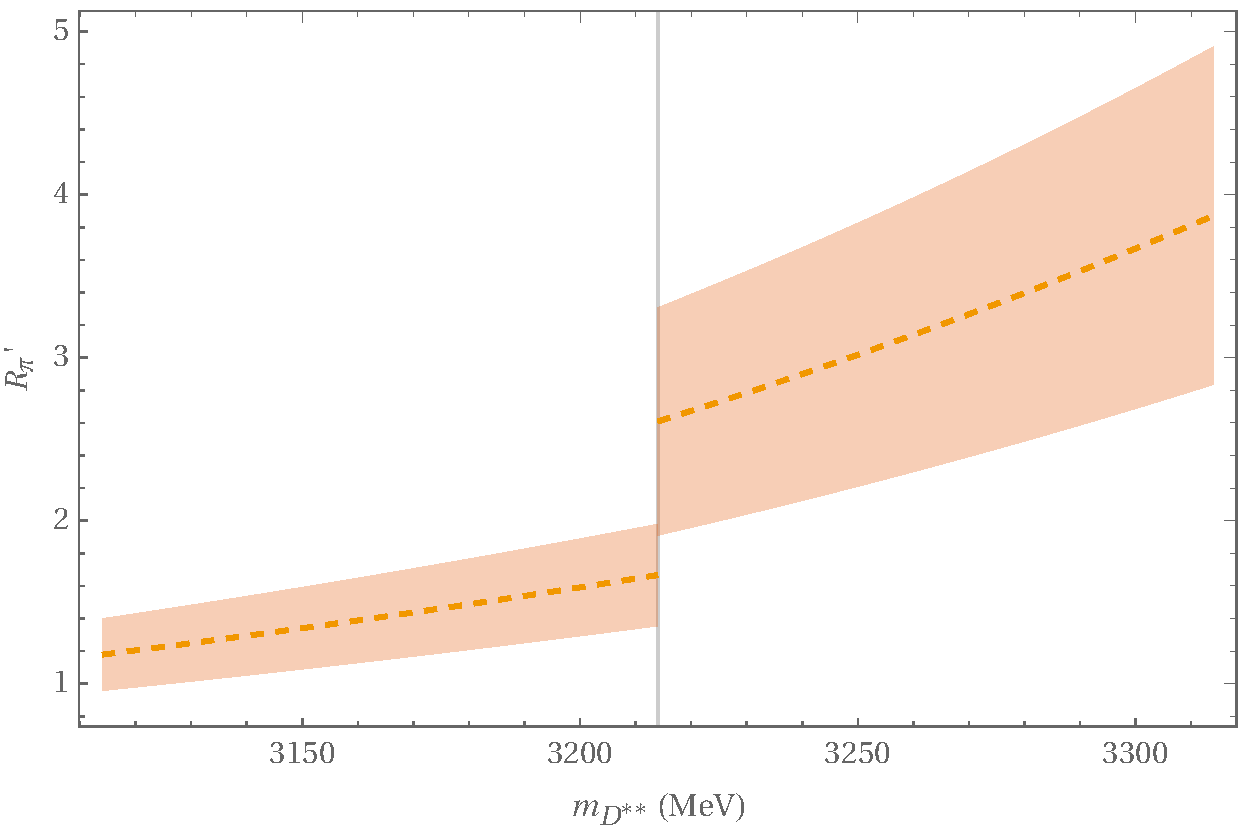
\includegraphics[width=0.8\textwidth]{figures/plot.pdf}
  \caption{Possible values of $R'_\pi$ against the mass of $D^{* \prime}_{s 2}$. The left-hand side refers to the case in which $D^*_2(3000)$ belongs to the $\tilde{T}$ doublet and $D^{**}$ is its spin partner with $J^P=1^+$. The right-hand side refers to the case in which $D_2^*(3000)$ belongs to the $F$ doublet and $D^{**}$ is its spin partner with $J^P=3^+$.}
  \label{fig:R'pi}
\end{figure}

Finally, the observation of the $D_2^*(3000)$ allows to draw further conclusions. Indeed, the strange partner of the $D^*_2(3000)$, namely the $D^{* \prime}_{s 2}$, should have mass of about $3.3 \ \text{GeV}$. This information can be used to calculate the analogous of equation \eqref{eq:Rpi_numeric} for decays of the $D^{* \prime}_{s 2}$ to a strange meson of the $H$ doublet plus $K$ or $\eta$. Such quantities are listed below, where I have assumed\footnotemark{} the value $3313 \pm 62 \ \text{MeV}$ for the mass of the $D^{* \prime}_{s 2}$
\footnotetext{It was used the following estimate
\begin{align*}
  m_{D^{* \prime}_{s 2}} &= m_{D^*_{s 2}(3000)} + \overline{\Delta m_s} \\
  \sigma \left( m_{D^{* \prime}_{s 2}} \right) &= \sqrt{\sigma \left( m_{D^{* \prime}_{s 2}(3000)} \right)^2 + \sigma \left( \Delta m_s \right)^2 }
\end{align*}
where $\overline{\Delta m_s}$ and $\sigma \left( \Delta m_s \right)$ are the weighted mean and standard deviation of the difference between the masses of $D$ mesons and their strange partner $m_s = m \left(D^{**}_s \right) - m \left( D^{**} \right)$, where $D^{**}$ are the $D(1869)$, the $D^*(2010)$, the $D^*(2600)$, the $D_1(2420)$, the $D^*_2(2460)$ and the $D^*_3(2760)$ (see table \ref{tab:charm_taxonomy}).}

\begin{subequations}
  \begin{align}
    R_K &= \frac{\Gamma \left( D_{s 2}^{* +} \rightarrow D^{* 0} K^+ \right) + \Gamma \left( D_{s 2}^{* +} \rightarrow D^{* +} K_S \right)}{\Gamma \left( D_{s 2}^{* +} \rightarrow D^0 K^+ \right) + \Gamma \left( D_{s 2}^{* +} \rightarrow D^+ K_S \right)} \ ,
    \quad
    R_K =
      \begin{cases}
        0.39 \pm 0.02 & F \\
        1.02 \pm 0.03 & \tilde{T} 
      \end{cases} \ , \\
    R_\eta &= \frac{\Gamma \left( D_{s 2}^{* +} \rightarrow D_s^+ \eta \right)}{\Gamma \left( D_{s 2}^{* +} \rightarrow D^0 K^+ \right) + \Gamma \left( D_{s 2}^{* +} \rightarrow D^+ K_S \right)} \ ,
  \quad
    R_\eta =
      \begin{cases}
        0.29 \pm 0.01 & F \\
        0.31 \pm 0.01 & \tilde{T} 
      \end{cases} \ , \\
    R^*_\eta &= \frac{\Gamma \left( D_{s 2}^{* +} \rightarrow D_s^{* +} \eta \right)}{\Gamma \left( D_{s 2}^{* +} \rightarrow D^0 K^+ \right) + \Gamma \left( D_{s 2}^{* +} \rightarrow D^+ K_S \right)} \ , 
   \quad 
    R^*_\eta =
      \begin{cases}
        0.10 \pm 0.01 & F \\
        0.29 \pm 0.02 & \tilde{T} 
      \end{cases} \ .
  \end{align}
  \label{eq:Rstrange}
\end{subequations}
It can be noticed that the most significant difference is found in the ratio $R_K$. Moreover, in the case $D^*_2(3000)$ belongs to the $F$ doublet the ratio $R_\eta^*$ is much smaller than $R_K$ and $R_\eta$, while in the event it belongs to the $\tilde{T}$ doublet the two ratios $R_\eta$ and $R_\eta^*$ are almost equal size and $R_K$ is much larger than the other two. These findings are summarized at the end of the chapter.

\section{Final remarks about $D_2^*(3000)$ decay modes}

The mass of $D^*_2(3000)$ is large enough to allow other decay modes besides those discussed in the previous section. For example, it can decay to members of doublets other than the $H$ doublet plus a light pseudoscalar meson. The features of such decay modes are different for the two assignments discussed in this thesis. One could argue that these modes are less important than the ones already considered, on the basis of the reduced phase space available for them. Moreover, their theoretical estimate would require the introduction of further coupling constants, at present unknown.

Other possible decay channels are those with the emission of a light vector meson, such as $D \rho$ or $D^* \rho$. In this case, the phase space would not be suppressed as in the case of decays to higher doublets and these modes cannot be neglected. Their estimate is possible using an approach similar to the one already exploited here. Indeed, an effective Lagrangian approach has been developed using the hidden gauge symmetry idea \cite{Bando:1985rf,Bando:1987br}. The description of this method is beyond the scope of this thesis. 

As a final remark, I would like to mention that, if the decay modes to $D\pi$ and $D^* \pi$ were the only relevant ones, it would have been possible to estimate the strong coupling constant appearing in the effective Lagrangian \eqref{eq:F_Lagrangian} in the two cases: by equating the theoretical expression of the decay widths to the experimentally measured total width one could have easily derived such a parameter and, consequently, it would have been possible to estimate the width of the spin partner. Due to the existence of the other decay modes mentioned above, this procedure could only lead to an upper bound on the strong coupling constant.

%I summarize below the main results that can allow to properly identify $D_2^*(3000)$.
\cleardoublepage
\vspace*{\fill}
\begin{center}
  \fbox{\begin{minipage}{\textwidth}
      {\Large \bfseries Summary of the Results for the Classification of the $D_2^*(3000)$} \\
    
    {\large \bfseries Case $D_2^*(3000)$ belongs to the $F$ doublet}
    \begin{itemize}
      \item Predicted ratio $R_\pi$ (defined in equation \eqref{eq:Rpi_formula}):
      \begin{equation*}
        R_\pi=0.40 \pm 0.01
      \end{equation*}
      \item Spin partner: $D_3^*$ with $J^P=3^+$. Should be looked for in the mass range $\approx 3.2\text{--}3.3 \ \text{GeV}$.
      \item Predicted  ratio $R_\pi^\prime$ defined in eq. (3.17):
      \begin{equation*}
        R_\pi^\prime=3.60 \pm 1.60
      \end{equation*}
      \item Predicted hierarchy for ratios $R_K,\ R_\eta, \ R_\eta^*$ for the strange partner (see equations \eqref{eq:Rstrange}):
      \begin{equation*}
        R_K > R_\eta \gg R_\eta^*
      \end{equation*}
      and, in particular
      \begin{equation*}
        R_K=0.39 \pm 0.02.
      \end{equation*}
    \end{itemize}
    
    {\large \bfseries Case $D_2^*(3000)$ belongs to the $\tilde{T}$ doublet}
    \begin{itemize}
      \item Predicted ratio $R_\pi$ (defined in eq. (3.15)):
      \begin{equation*}
        R_\pi=1.06 \pm 0.03
      \end{equation*}
      \item Spin partner: $\tilde{D}_1$ with $J^P=1^+$. Should be looked for in the mass range $\approx 3.1\text{--}3.2 \ \text{GeV}$.
      \item Predicted  ratio $R_\pi^\prime$ defined in eq. (3.17):
        \begin{equation*}
          R_\pi^\prime=1.50 \pm 0.60
        \end{equation*}
      \item Predicted hierarchy for ratios $R_K,\ R_\eta,\ R_\eta^*$ for  the strange partner (see equations \eqref{eq:Rstrange}):
      \begin{equation*}
        R_K \gg \ R_\eta \approx R_\eta^*
      \end{equation*}
      and, in particular
      \begin{equation*}
        R_K=1.02 \pm 0.03.
      \end{equation*}
    \end{itemize}
  \end{minipage}}
\end{center}
\vspace*{\fill}

% vim: ft=tex nonumber wrap linebreak display+=lastline guifont=Inconsolata\ 20 spell spelllang=en_gb
